\documentclass[sigconf,nonacm]{acmart}
\settopmatter{printacmref=false}
\renewcommand\footnotetextcopyrightpermission[1]{}
\pagestyle{plain}
\newcommand{\validruns}{23}
\newcommand{\invalidruns}{0}

\usepackage{booktabs}
\usepackage{tikz}
\usetikzlibrary{arrows.meta,positioning}
\setlength{\textfloatsep}{6pt plus 2pt minus 2pt}
\setlength{\floatsep}{6pt plus 2pt minus 2pt}
\setlength{\intextsep}{6pt plus 2pt minus 2pt}

\begin{document}

\title{\texttt{parbench}: Measuring How Coding-Agent Harnesses Handle $k$ Concurrent, Conflicting Tasks}
\subtitle{Mid-Submission Progress Report (Phase 2)}

\author{Vishesh Saraswat}
\author{[Teammate 2]}
\author{[Teammate 3]}
\affiliation{\institution{IIIT Hyderabad}\country{India}}
\begin{abstract}
Parallel coding agents waste compute when tasks touch the same files: they re-explore the same context, overwrite each other and produce changes that no longer merge. No benchmark measures this beyond two tasks. We are building \texttt{parbench}, a pipeline that bundles $k$ tasks from CooperBench into one repository snapshot, runs them under different orchestration strategies and harnesses, grades every task on the final tree, and logs tokens, time and conflicts. This report covers the architecture, the decisions made, the experiments run so far (Gemini and GPT-OSS through Antigravity, Qwen2.5-7B through OpenCode, a toy pool), the problems we hit, and the remaining work. Results are preliminary: small $n$, one repeat.
\end{abstract}
\maketitle

\section{Problem and Motivation}
Coding agents are now used on several tasks at once, by fanning out to subagents or by running one agent per task. When the tasks overlap, uncoordinated agents duplicate exploration, overwrite one another and produce patches that conflict at merge time. CooperBench~\cite{cooperbench} showed that two cooperating agents do worse than one agent doing both tasks, but it covers only pairs, one harness and a hand-built dataset. No benchmark lets us ask how orchestration strategy, harness and model affect \emph{correctness, cost and wasted effort} as the number of concurrent tasks $k$ grows. Our goal (Phase~1 proposal) is a benchmark and evaluation pipeline for exactly this, built on existing datasets and existing harnesses; we do not train a model or write a new agent framework.

\section{System and Architecture}
\textbf{Vocabulary.} A \emph{task} is one CooperBench feature with hidden tests; a \emph{pool} is the set of tasks sharing one repository at one base commit (CooperBench calls the pool a ``task'' and our task a ``feature''); a \emph{bundle} is $k$ tasks from one pool in a fixed seeded order; a \emph{run} is bundle $\times$ strategy $\times$ harness $\times$ model $\times$ repeat. CooperBench has 30 pools, 199 tasks and 652 pairs; we use its curated \texttt{core} subset (10 pairs, 9 repositories, four languages).

\textbf{Pipeline} (\texttt{src/parbench}, about 2.7k lines of Python, 34 commits from three contributors). (1) A bundle sampler builds $k$-task bundles. For $k>2$ it extends each curated pair with more tasks from the same pool. (2) Each agent starts in a clean copy of the repository with the history after the base commit removed (CooperBench images contain the upstream future commits). (3) A strategy runs the agents. (4) If an agent ends by asking a question it is resumed with ``No human is available; use your best judgement'' (counted as a nudge). (5) We collect each agent's diff ourselves. (6) A grader applies the final tree, as one diff against the base, and runs each task's hidden tests with the pool image's own \texttt{runner.sh}; a task passes only if the runner exits 0 and at least one test passed. CooperBench's grader handles two features only, so ours handles any $k$. (7) A record per run stores correctness, tokens, wall-clock time, agent-busy time, conflicts, overlap and per-agent logs.


\begin{figure}[t]
\centering
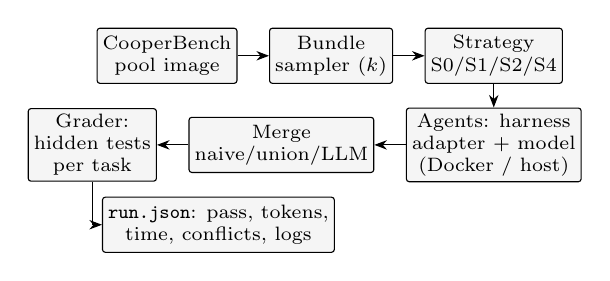
\begin{tikzpicture}[font=\scriptsize, node distance=3mm and 4mm,
  box/.style={draw, rounded corners=1pt, align=center, minimum height=7mm, inner sep=2pt, fill=gray!8},
  arr/.style={-{Stealth[length=1.6mm]}}]
\node[box] (pool) {CooperBench\\pool image};
\node[box, right=of pool] (bun) {Bundle\\sampler ($k$)};
\node[box, right=of bun] (strat) {Strategy\\S0/S1/S2/S4};
\node[box, below=of strat] (ag) {Agents: harness\\adapter + model\\(Docker / host)};
\node[box, left=of ag] (merge) {Merge\\naive/union/LLM};
\node[box, left=of merge] (grade) {Grader:\\hidden tests\\per task};
\node[box, below=of merge, xshift=-8mm] (rec) {\texttt{run.json}: pass, tokens,\\time, conflicts, logs};
\draw[arr] (pool)--(bun); \draw[arr] (bun)--(strat); \draw[arr] (strat)--(ag);
\draw[arr] (ag)--(merge); \draw[arr] (merge)--(grade); \draw[arr] (grade)|-(rec);
\end{tikzpicture}
\caption{The \texttt{parbench} pipeline. Every agent starts from a clean copy of the pool image with later upstream history removed.}
\label{fig:pipe}
\end{figure}

\textbf{Strategies.} S0 runs each task alone (the $k{=}1$ reference for retention). S1 gives one agent all $k$ tasks. S2 runs one agent per task in parallel and merges the patches in three modes: plain \texttt{git merge}, git's union driver, and an LLM resolver that is the same agent. S4 gives all tasks to a harness with its native subagents enabled, in a variant where the lead agent also does the merging in git worktrees. Prompt variants (plan first, other tasks visible) are in place; a planner-based strategy (S3) is not built yet.

\textbf{Harnesses.} Adapters exist for OpenCode, Pi, Claude Code, Codex CLI, Antigravity (\texttt{agy}) and Gemini CLI; each writes its own config, runs headless with JSON output, and a parser converts tokens to a common convention (input including cached tokens). Only OpenCode and \texttt{agy} have been checked against real output so far.

\textbf{Sandbox.} Agents run in Docker containers built from the CooperBench pool image, so they can run the project's own tests. A host mode (temporary clone, no Docker) exists for \texttt{agy} and for OpenCode; a teammate added a second no-Docker route using prepared host directories for use on a GPU machine.

\section{Decisions Made}
\begin{itemize}\itemsep0pt
\item \textbf{Build on CooperBench} (pinned submodule, commit \texttt{63b9d44}) and re-bundle it, instead of writing tasks by hand.
\item \textbf{Strategies first}: S0, S1, S2, S4. Teammates' literature notes are treated as guidance, not a specification.
\item \textbf{Docker sandbox per agent} and agents may run the repository's tests; hidden tests are never visible.
\item \textbf{Fully autonomous agents}: no human in the loop, resumed with a fixed nudge, up to two times.
\item \textbf{Compute}: local Ollama on a 24~GB Mac for smoke tests; a GPU machine with vLLM for the main OpenCode runs (run by a teammate on another machine); Antigravity for hosted Gemini and GPT-OSS. The team accepted the terms-of-service risk of scripting \texttt{agy} on a personal account at low concurrency.
\item \textbf{Fairness}: same model for agents, resolver and planner; same step limit; one seeded task order per bundle.
\item \textbf{Everything is logged raw} (JSON from each harness), so parsers can be fixed and runs re-scored without re-running agents.
\end{itemize}

\section{Experimental Setup}
\textbf{Datasets.} (a) A toy pool (6 features of a small Python package, known conflict structure) to check the pipeline. (b) CooperBench \texttt{core}: five Python/Go pools so far (dspy~8563, go\_chi~27, click~2800, jinja~1559 and~1621), $k{=}2$, one repeat. \textbf{Grader check.} For 41 real features in six pools, the tests fail on the base, the gold patch passes, and CooperBench's combined patch passes, on arm64 images; likewise for the six toy features.
\textbf{Models and harnesses.} \texttt{agy} with Gemini~3.8~Flash (low) and GPT-OSS~120B; OpenCode with Qwen3.5-9B (Ollama, thinking off, 64K context) on the toy pool and with Qwen2.5-7B-Instruct (vLLM, one RTX~5000 Ada; teammate, partial) on the Python pools of \texttt{core}.
\textbf{Metrics.} Task pass rate, bundle success, retention versus S0, pairwise conflict rate, overlap, tokens, wall-clock and agent-busy time, effective parallelism, nudges, and a validity flag. No dollar cost is computed for subscription models.

\section{Results (Preliminary)}
\textbf{Toy pool, OpenCode + Qwen3.5-9B (local).} All strategies pass all tasks: S0 $k{=}2$ (938\,s), S1 (536\,s), S2 (592\,s, all three merge modes), S0 $k{=}3$ (1312\,s). The bundle used had no conflicting pair, so the conflict path of the resolver was not exercised. These runs show the pipeline works end to end; they are not results.

\begin{table}[t]
\caption{\texttt{agy} on CooperBench \texttt{core} (5 pools, $k{=}2$, valid runs only, as of 6 Nov, 22:30 IST; runs still in progress). Task pass = mean fraction of the two tasks passing; Bundle = both pass; wall and tokens are medians per run.}
\label{tab:agy}
\small
\begin{tabular}{@{}llrcccc@{}}
\toprule
Model & Strat. & $n$ & Task pass & Bundle & Wall (s) & In-tokens (M) \\
\midrule
Gemini 3.8 Flash & S0 & 5 & 0.60 & 0.20 & 1350 & 16.0 \\
Gemini 3.8 Flash & S1 & 5 & 0.70 & 0.40 & 554 & 6.8 \\
Gemini 3.8 Flash & S2 & 3 & 0.83 & 0.67 & 643 & 8.7 \\
Gemini 3.8 Flash & S4 & 1 & 0.50 & 0.00 & 339 & 3.3 \\
\midrule
GPT-OSS 120B & S0 & 3 & 0.33 & 0.00 & 1255 & 6.3 \\
GPT-OSS 120B & S1 & 2 & 0.00 & 0.00 & 357 & 2.3 \\
GPT-OSS 120B & S4 & 2 & 0.00 & 0.00 & 188 & 1.0 \\
\bottomrule
\end{tabular}

\end{table}

\textbf{Antigravity, \texttt{core}.} Table~\ref{tab:agy} shows \validruns{} valid runs. With Gemini, S1 (one agent, both tasks) passes slightly more than S0 (0.70 vs.\ 0.60, $n{=}5$) and, because the isolated reference runs two agents, uses 2.4$\times$ fewer input tokens (6.8M vs.\ 16.0M) and less than half the wall-clock time (554\,s vs.\ 1350\,s). S2 passes 0.83 ($n{=}3$) with a pairwise conflict rate of 0.33 and an effective parallelism of 1.56; S4 has one valid run so far. The differences are not statistically meaningful at this $n$. GPT-OSS results are dominated by service failures (below) and say little about the model. A single task costs 3--8M input tokens, far above our initial estimate.


\begin{table}[t]
\caption{Task pass fraction per pool (valid runs; 1.0 = both tasks pass, -- = no valid run yet).}
\label{tab:pool}
\scriptsize
\begin{tabular}{@{}lcccccccc@{}}
\toprule
 & \multicolumn{4}{c}{Gemini 3.8 Flash} & \multicolumn{4}{c}{GPT-OSS 120B} \\
\cmidrule(lr){2-5}\cmidrule(lr){6-9}
Pool & S0 & S1 & S2 & S4 & S0 & S1 & S2 & S4 \\
\midrule
dspy 8563 & 0.5 & 0.5 & 0.5 & 0.5 & 0.0 & -- & -- & 0.0 \\
go\_chi 27 & 0.5 & 0.5 & 1.0 & 0.5 & 0.5 & -- & -- & -- \\
click 2800 & 0.5 & 0.5 & 0.5 & -- & 0.0 & 0.0 & 0.5 & -- \\
jinja 1559 & 0.5 & 1.0 & 1.0 & 1.0 & 0.5 & 0.0 & 0.0 & 0.0 \\
jinja 1621 & 1.0 & 1.0 & 0.5 & 1.0 & -- & -- & -- & -- \\
\bottomrule
\end{tabular}

\end{table}

\textbf{Per-pool view.} Table~\ref{tab:pool} shows the pattern behind the averages. With Gemini, the jinja~1621 pair passes both tasks in S0 and S1, while the dspy, go\_chi and click pairs pass exactly one of two in S0 and S1: one task per pair is consistently out of reach for this setup, whatever the strategy. We have not yet inspected which task fails or why. Because the agents could not run the repository tests on the host, some failures may be unverified mistakes, not missing capability.

\textbf{OpenCode + Qwen2.5-7B (teammate, partial, Python pools).} Across S0, S1 and S2 ($n{=}11,11,9$) no task has passed (0.00, 95\% CI up to 0.15--0.18), with and without a ``small model'' prompt. We cannot yet tell whether the model is too weak for these tasks (CooperBench reports weak results for small open models) or whether part of the no-Docker setup is at fault; this is the first thing to investigate.

\section{Problems Faced}
\begin{itemize}\itemsep0pt
\item \textbf{Dataset mismatch.} CooperBench's grader and runner handle two features and pass patches through one shell argument (large merged patches break); we wrote our own $k$-task grader and copy files with \texttt{docker cp}. Its images also contain future upstream commits, so we remove them before agents start.
\item \textbf{Local serving.} Ollama's default 4K context silently truncates prompts; a thinking model took more than five minutes per call (fixed with reasoning off); Ollama serves requests one at a time on the Mac, so parallel timings measure a queue; a \texttt{keep\_alive} bug broke the warm-up script.
\item \textbf{Docker.} Docker Desktop had 3.8~GB of RAM, too little for large pools; its settings file is ignored, so the limit had to be raised in the UI.
\item \textbf{Harness quirks.} OpenCode~2.x needs an explicit model map for custom providers (and differs from~1.x); \texttt{agy} rejects prompts passed in the wrong flag order, denies tool calls headless unless allowed, has no switch to disable subagents, and its login cannot be carried into a container, so it runs on the host.
\item \textbf{Safety and privacy.} A host-mode agent ran \texttt{env} and wrote the shell environment (session tokens) into a log. We redacted the logs before committing and now pass only an allow-list of environment variables.
\item \textbf{Benchmark contamination.} \texttt{agy} agents used web search to look for the upstream pull request behind the task (\emph{e.g.}, \texttt{site:github.com/pallets/click/pull/2800}). Deny rules did not block it, so we run \texttt{agy} with custom agents without web, browser and question tools, and an audit command flags any web use. 18 early runs were archived as contaminated and rerun.
\item \textbf{Quota and capacity.} After about 216M Gemini input tokens the account hit a quota limit (429) and GPT-OSS returned 503 ``no capacity'' errors; 23 of 42 runs ended on a service error and are excluded and rerun. The runner now waits and resumes, and marks such runs invalid.
\item \textbf{Scale.} The full benchmark at $k{=}2$ alone is 3,912 agent sessions (about 70,000 over all $k$), so we use curated subsets.
\item \textbf{Process mistakes} we corrected: broad process-kill patterns that killed our own watchers, deleting live temporary clones, and editing prompt templates while an experiment was running.
\end{itemize}

\section{Limitations}
$n$ is tiny and each configuration has one repeat; confidence intervals are wide. \texttt{agy} runs on the host, so agents cannot run the repository's tests, which lowers absolute pass rates and makes them not directly comparable with containerised OpenCode runs; subagents cannot be disabled in \texttt{agy} S0--S2 apart from our custom agent. Model quotas and server capacity are outside our control. Only $k{=}2$ has been run, and only one harness has results on real pools with a model strong enough to pass tasks.

\section{Remaining Work (to 30 November)}
\begin{itemize}\itemsep0pt
\item Finish the \texttt{core} runs (S4 and the heavy pools: outlines, typst, tiktoken, llama\_index, react-hook-form) and add repeats ($\ge$3) with confidence intervals.
\item The main OpenCode experiments on a GPU machine with a stronger open model (Qwen 27B--35B class), and find out why Qwen2.5-7B passes nothing.
\item $k=3,4,6$ bundles and an analysis by conflict density using CooperBench's gold conflict report.
\item Validate the Pi, Claude Code and Codex adapters on real output; cache S0 results across bundles.
\item Our own contribution: a predict-then-schedule strategy (S3) that predicts each task's files, runs conflicting tasks one after another and the rest in parallel, evaluated with file-prediction recall and the cost saved.
\item Report cost and resource use (tokens, GPU-hours) as in the proposal, and the final ACM-format report.
\end{itemize}

\section{Use of AI Tools}
Most of the pipeline code, documentation and this draft were written with Claude Code (Claude Opus~5.5 and Sonnet~5.5), including delegated research subagents; AI agents are also the subjects of the experiments (Gemini, GPT-OSS, Qwen via OpenCode and \texttt{agy}). Outputs were verified by running the grader on gold patches, dry-running experiment plans, inspecting run logs, and review of every commit. \textbf{[Team: attach prompt log and list how each person verified or changed AI-written parts.]}

\section*{Repository}
\url{https://github.com/vishesh312/autose-project} \textbf{[currently private: grant TA/instructor access or make public]}. The history has 34 commits from three contributors over 4--6 November (pipeline, adapters, documentation, and a teammate's GPU-machine runs with automated result publishing). Start with \texttt{AGENTS.md}, \texttt{docs/findings.md} and \texttt{docs/core\_subset\_plan.md}.

\begin{thebibliography}{9}
\bibitem{cooperbench} CooperBench: benchmarking coding-agent cooperation. arXiv:2601.13295, 2026 (code: github.com/cooperbench/CooperBench).
\end{thebibliography}

\end{document}
